\documentclass[times, 10pt,onecolumn]{article} %
\usepackage{latex8}
\usepackage{times}
\usepackage{url}
\usepackage{amsmath}%
\usepackage{amsfonts}%
\usepackage{amssymb}%
\usepackage{graphicx}
\usepackage{cases}
\usepackage{algorithmic}

%\usepackage{amsfonts, amsthm}

\title{Service-oriented Local and Global Visualization with Sorting On-demand for Climate Data}
\author{
Xusheng Xiao\\
\small{xxiao2@ncsu.edu}\\
\small{Nov 27th, 2010}
}

\begin{document}
\maketitle
\abstract
\textit{Huge amount of climate simulation data are collected from different areas (e.g., cities, countries). By understanding and analyzing the data, climate scientists try to predict the trends of the variation of climate both locally and globally. To assist the prediction, exploring visualization of data mining (e.g., histogram) has been used more and more frequently to get a general view ahead of predicting. Additionally, climate experts would like to analyze data by navigating among levels of data ranging from the most summarized (drill-up) to the most detailed (drill-down). To achieve local and global visualization of climate data, there are two major challenges: (1) globally tranferring data is time-consuming and (2) frequently drill-up and drill-down navigation requires computation of same data set multiple times. To address these challenges, we propose a service oriented approach to compute local and global visualization with sorting on-demand for climate data. For global transferring data, our novel approach first asks the data sources to compute local parameters (min, max and count). By collecting these local parameters, our approach computes global parameters and distribute these global parameters to guide local data sources how to compute the histogram data using proper parameters. These computed histogram data from different data sources are then transferred to form a global histogram, whose size is much less than the whole data sets. For data navigation of historgram, our approach caches the transferred data sets and sort only the data in the interval later requested by the data navigation. In this way, we enable climate scientists to navigate huge data sets with acceptable performance. Our preliminary results show that our approach can perform well on sample data sets of climate simulation data.  
}\endabstract

\section{Introduction}
\subsection{Motivations} 
Increasing computing power enables modelers to generate larger simulation data sets of climate data from different areas (e.g., cities, countries and continents). Identifying and analyzing patterns in these data sets of climate simulatin data is important, since these patterns help climate scientists develop a deeper understanding of the complex processes contributing to observed phenomena. By understanding and analyzing these data sets of climate data, climate scientists can predict the trends of the variation of climate both locally and globally. 

\begin{figure}[!iht]
\begin{center}
  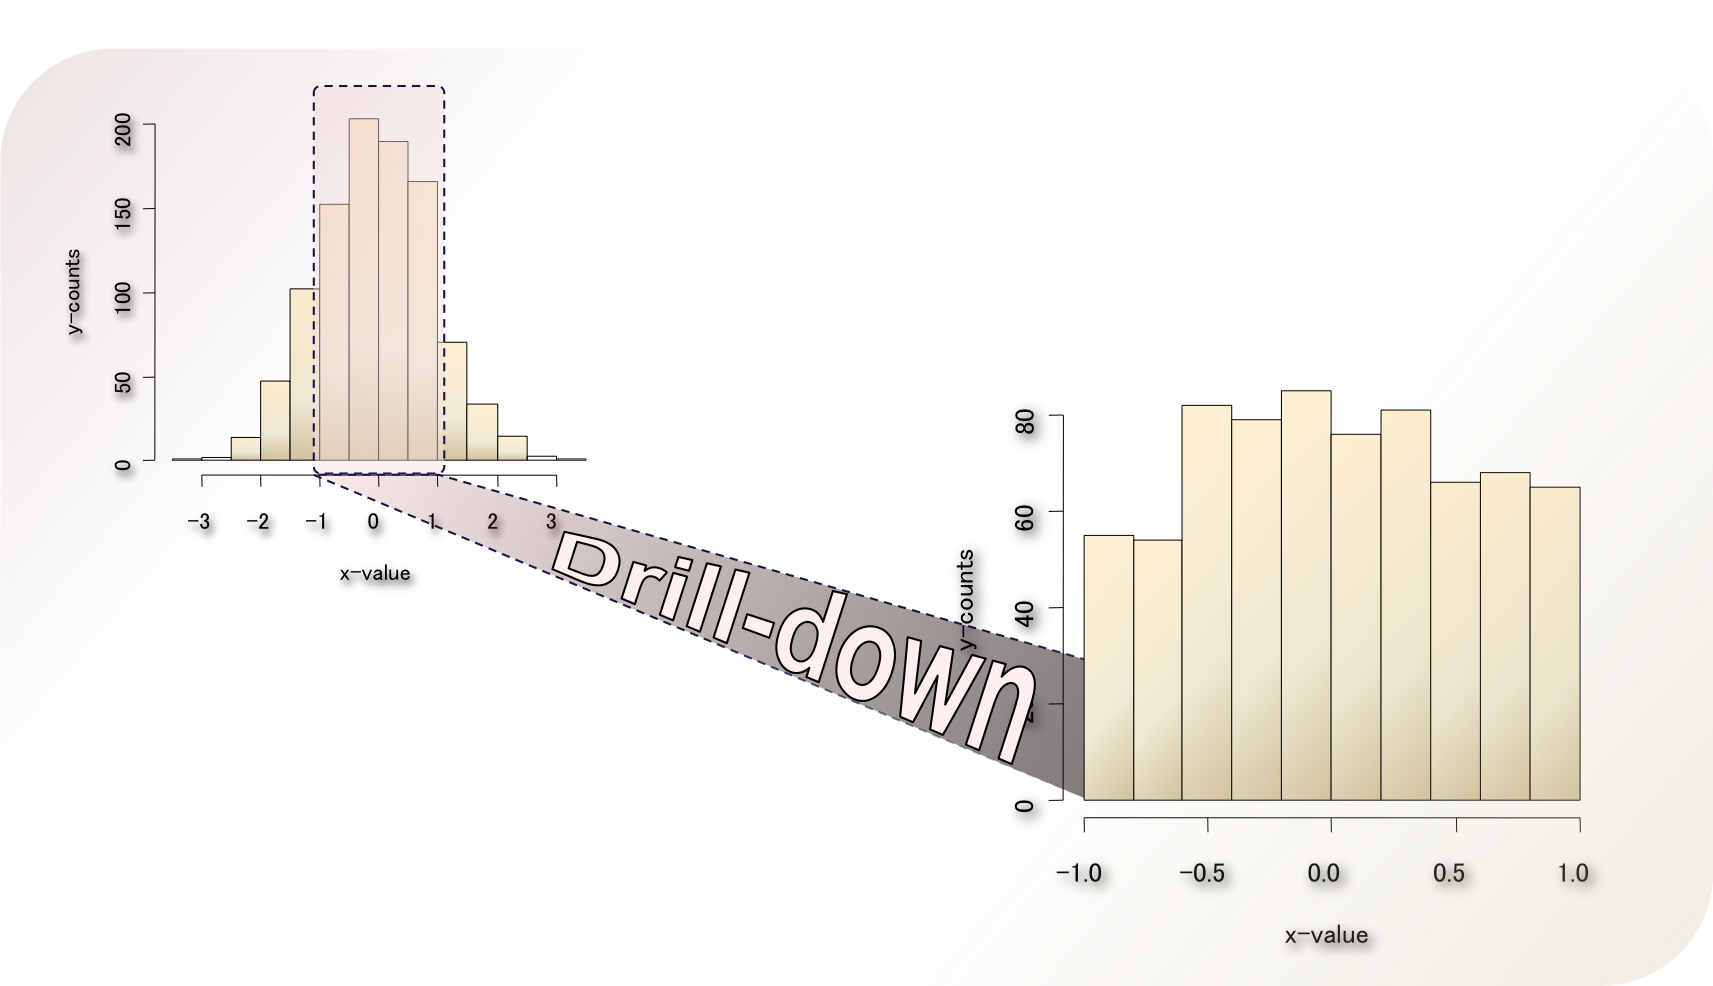
\includegraphics[scale=0.45]{drill.png}
  \caption{Drill-down to interval [-1,1] in histogram}
  \label{fig:drill}
\end{center}
\end{figure}

In order to assist the prediction of the climate variation, exploring visualization of data mining (e.g., histogram~\cite{histogram}) has been used more and more frequently. Showing a global histogram of climate simulation data collected from different data sources can help climate scientists obtain a general view ahead of predicting. However, climate data is well known for its huge amount. In every second, huge amount of climate simulation data is generated from different cities, countries or even thousands of sensors in the same area. The computation for global visualization using histogram normally depends on the distributed computation on different data sources. Hence, there is much need of transferring huge data sets from different data sources with acceptable error rate for computing global visualization. 

%\usepackage{graphics} is needed for \includegraphic

Moreover, to better understand the details of specific areas, climate experts would like to analyze data by navigating among levels of data ranging from the most summarized (drill-up) to the most detailed (drill-down), analogous to navigation in data cube~\cite{datamining}. As we can see in Figure \ref{fig:drill}, the left histogram shows a better global generalization of the distribution of the whole dataset, whereas the right histogram demonstrates a better detailed visualization of the distribution for data with x-value ranges from -1.0 to 1.0. 

\subsection{Challenges} 
In order to visualize climate data sets locally and globally with acceptable performance, there are two major challenges. The first challenge is the high computation time and the unacceptable package loss rate during the global data transferring. Table \ref{tbl:rawdata} shows the synopsis of raw climate data in multiple domains dollected in 2008. As we can see for the data of VOCALS in the table, the data size in 2008 is 3920 MB and transferring this data set requires 10 hours even in best case.

\begin{table}[!iht]
\centering
\begin{tabular}{|c|c|c|c|c|}
\hline
\textbf{Data Domain} & \textbf{Single data set size} & \textbf{\# data sets} & \textbf{Total Size} & \textbf{ Transfer Time In Best Case (Hrs)} \\ \hline
VOCALS 2008 & $\sim$70000 KB & 56 & $\sim$3920 MB & $\sim$10 \\ \hline
HrsASCOS 2008 & $\sim$140000 KB & 25&  $\sim$3500 MB & $\sim$10 \\ \hline 
HrsAEROSE 2008 & $\sim$80000 KB & 36&  $\sim$2880 MB & $\sim$7 \\ \hline 
HrsSTRATUS 2007 & $\sim$70000KB & 21&  $\sim$1470 MB & $\sim$5  \\ \hline
\end{tabular}
\caption{The synopsis of raw climate data in multiple domains collected in 2008.}
\label{tbl:rawdata}
\end{table}

Another challenge is the frequent data navigation of climate data. By drilling-up or drilling-down of the global histogram, we need to recompute the data sets in the specified range, which requires re-transferring the whole data if traditional approach is used. However, Table \ref{tbl:rawdata} already shows that tranferring whole data sets require non-trivial time. Thus, re-transferring whole data set for a navigation is unacceptable. Table \ref{tbl:time} further shows the detailed computation time needed to discovery meaningful or user-specified parameters visualization. As we can see in the table, for the data set of size about 3000 MB, it requires 4 minutes to compute a histogram and 30 times requires 120 minutes, which is far from acceptable performance. 


\begin{table}[!iht]
\centering
\begin{tabular}{|c|c|c|c|}
\hline
\textbf{Data Size} & \textbf{Histogram Execution Time (Once) } & \textbf{Discovery Histogram Execution Time (log(n))} & \textbf{User-specified (30 Times)} \\ \hline
$\sim$1500 MB & 2 Mins & $\sim$17 * 2 = 34 Mins & 60 Mins \\ \hline
$\sim$3000 MB & 4 Mins &  $\sim$18 * 2 = 36 Mins & 120 Mins \\ \hline 
$\sim$4500 MB & 6 Mins &  $\sim$19 * 2 = 38 Mins & 180 Mins \\ \hline 
\end{tabular}
\caption{Total time needed to discovery meaningful or user-specified parameters visualization.}
\label{tbl:time}
\end{table}

\subsection{Solution}
To address these two major challenges, we provide a novel approach, called Service-oriented Local and Global Visualization with Sorting On-demand for Climate Data. Basically, our approach consists of two major steps: 

\begin{itemize}
\item{\textbf{Part I: Service-Oriented Histogram.}} Instead of transferring the whole data sets from different data sources, our approach first locally compute the parameters (min, max and total count of sample data points) based on the requirements of a histogram request. These local data sources then communicates with each other to further compute regional parameters. These regional parameters are processed to compute the global parameters and then re-distribute to each data source for computing the required data sets of local histograms. These local histograms based on the global parameters, whose size is much less than the whole data sets, are finally transferred to compute the global histogram.
\item{\textbf{Part II: On-demand Sorting.}} After transferring the required data sets of local histogram, each data source caches the data sets. When further data navigation requests come in, each data source sorts only the data in the intervals based on the request and recompute a local histogram. These recomputed local histograms are again sent to form a global histogram that fulfills the navigation requirement. 
\end{itemize}


\section{Preliminary Materials and Approaches}
\subsection{Data Description}
The Radar Data Information of those projects are stored on a Tb data storage system at PSD in Boulder, CO\footnote{\url{http://www.esrl.noaa.gov/psd/psd3/cruises/}}. The details of data is shown as below.
\begin{itemize}
  \item \textbf{VOCALS 2008:} 915 MHz profiler reflectivity from vertical pointing beam only. These data are from the electronically stabilized system. 
\item \textbf{ASCOS 2008:} 449 MHZ Wind Profiler data; half-hour consensus profile data from the 449 MHz wind profiler on the Oden during ASCOS.  
\item \textbf{AEROSE 2008:} 556 MHZ Wind profiler rbclear AEROSE 2008, one-hour consensus profile data.
\item \textbf{STRATUS 2007:} 778 MHZ Wind profiler rcSNR AMMA 2007, UTC time per hour consensus profile data.
\end{itemize}
\subsection{Data Transmission and Package Loss Ratio}
\textbf{Data transmission, digital transmission or digital communications} is the physical transfer of data (a digital bit stream) over a point-to-point or point-to-multipoint communication channel. Examples of such channels are copper wires, optical fibers, wireless communication channels, and storage media. The data is represented as an electromagnetic signal, such as an electrical voltage, radio-wave, microwave or infrared signal~\cite{PDAT}. 

\textbf{Package Loss} occurs when one or more packets of data travelling across a computer network fail to reach their destination. Packet loss is distinguished as one of the three main error types encountered in digital communications; the other two being bit error and spurious packets caused due to noise\footnote{\url{http://www.nessoft.com/kb/24}}.
\subsection{Histogram}
\subsection{Sort\cite{ps}}

\section{Our Approach}
Figure \ref{fig:overview} shows the overview of our approach. Generally, our approach consists of two major components: \textbf{Service-Oriented Histogram} and \textbf{On-demand Sorting}. In the figure, Region 1 demonstrates the procedure of Service-Oriented Histogram and Region 2 illustrates the procedure of Service-Oriented Histogram integrated with On-demand Sorting.

\begin{figure}[!iht]
\begin{center}
  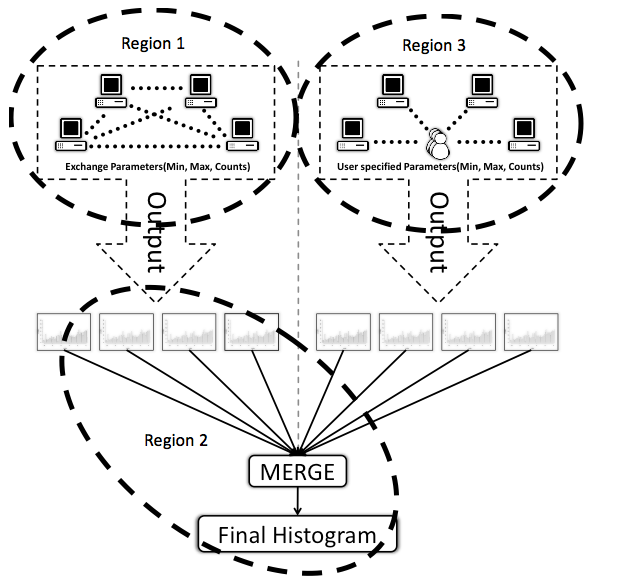
\includegraphics[scale=0.65]{architecture.png}
  \caption{Overview of Our Approach}
  \label{fig:overview}
\end{center}
\end{figure}

\subsection{Service-Oriented Histogram}
Global visualization of datasets requires accurate data from every source. To compute a global histogram, the data is collected distributedly from thousands of sources. Traditional approach simply uses a central computer to calculate all the collected date transferred from thousands of sources, which heavily relies on the data transfer of whole data sets from different data sources, which is shown to be challenging in Section 1.2 due to time-consuming data transfer and unacceptable package loss. Another traditional approach let the data sources compute their local histogram and then uses a central computer to integrate all the local histogram, rather than using a central computer to calculate all the collected raw date. This approach shows a little improvement. However, since the climate data collected from different dat sources usually varies a lot in terms of parameters (min, max and total count of sample data points), the local histogram cannot be used directly for merging a global histogram. Therefore, it still cast another burden on the central computer, which is how to fast coordinate different parameters such as min, max, and count among thousands of histograms.

To address these issues, we advocate a novel approach, called \textbf{Service-Oriented Histogram}. Service-oriented histogram borrows the ideas from Service-Oriented Architecture (SOA)~\cite{soa}. In SOA, each component of the system is integrated as an individual service. Services have control over the logic they encapsulate (service autonomy). There are many benefits for this approach: The first benefit from such design principle is that SOA maximizes the reuse of services. Another benefit is that the service autonomy realizes the loose coupling among services which makes the global system more robust. Borrowing these concepts, instead of computing the global histogram in one central node, service-oriented histogram computes local histograms based on the computed global parameters and merge to form a global histogram. 

To address the challenge of transferring whole data sets of climate data from different data sources, our approach let the data sources compute their local histograms. Moreover, to relieve the burden of the central computer for coordinating different parameters, we perform a global parameter computation before the data sources computing their local histograms. As shown in the Region 1 in Figure \ref{fig:overview}, before transferring their data to central computer, each data source computes its own parameters (min, max and count) and transmit its local parameters to all the others in the same region in order to compute global parameters. These regional parameters are further transferred to the central computer to finalize the global parameters. The global parameters are then re-distributed to each data source, guiding these data sources to compute local histograms.

With the guidance of global parameters, each data source computes local histogram using the global paramaeters. In this way, we can only transfer the computed histrogram data rather than the whole data sets of climate data. Finally, since these local histograms are based on the same global parameters, the central computer directly merge the received local histograms to form the global histograms, shown as Region 2 in Figure \ref{fig:overview}.


\subsection{On-demand Sorting}
\textbf{On-demand Sorting} is another improvement of our service-oriented histogram approach. It is specially designed to meet the needs of users such as climate scientist who would like to analyze data by navigating among levels of data ranging from the most summarized (drill-up) to the most detailed (drill-down). 

When drill-up or drill-down is performed on the global histogram, re-transferring the whole data sets of climate data is required since the global histogram does not have the detailed enough data or lacks of more summarized data. To prevent re-transferring the whole data sets of climate data, we can re-apply service-oriented histogram approach described in Section 3.1. However, directly applying service-oriented histogram approach still requires re-computation of the same data, which reduces the performance gain when data navigation of global histogram is frequent.

To address this issue, we propose another improvement approach, called On-demand Sorting. On-demand sorting requires each data source to cache the transferred data sets in the form of computed local histogram using global parameters. That is to say, if the computed local histogram has 50 sample points falling into the interval of [-1, 0], then these 50 data points shall be kept in one cache region instead of spreading into several regions. The benefits of this caching is we can sort only the data inside the interval requested by the data navigation instead of sorting all the data and re-computing the whole data sets.  

Region 3 in Figure 2 illustrates the whole procedure of service-oriented histogram integrated with on-demand sorting: local sources first cache data and parameters (min, max, count) and index data with break number (e.g., 0.5 is in the break [0, 1] ); When users specify a certain interval, local sources check whether the data in the requested breaks are sorted or not; If data is already sorted, our approach transfers data directly to the central computer; If data is not sorted, our approach sorts only the data in the corresponding break and mark the break as sorted; Then our approach transfers local histogram data (min, max, count) to the central computer; Finally, the central computer merges data from different sources and form a global historgram that fulfills the requirements of data navigation.


\section{Preliminary Result}

We conduct experiments to compare the performance of three histogram approaches: Traditional Histogram, Service-Oriented Histogram, and Service-Oriented Histogram with On-demand Sorting. Below we describe the experiment procedures in detail.

\begin{enumerate}
\item{Traditional Histogram:} Collect all data sets into a central computer and execute original histogram multiple times to compute the results of discovery histograms. Table \ref{tbl:1stStr} shows the details of the results.

\begin{table}[!iht]
\centering
\begin{tabular}{|c|c|c|c|p{3cm}|}
\hline
\textbf{Data Domain} & \textbf{Total Size} & \textbf{ Data Transfer Time (Hrs)} & \textbf{Discovery Histogram (Mins)} & \textbf{Total Execution Time (Hrs)}  \\ \hline
VOCALS 2008 &  $\sim$3920 MB & $\sim$10 & $\sim$37& $\sim$10.6\\ \hline
ASCOS 2008 & $\sim$3500 MB & $\sim$10 & $\sim$36& $\sim$10.5\\ \hline 
AEROSE 2008 & $\sim$2880 MB & $\sim$7 & $\sim$35&  $\sim$7.5 \\\hline 
STRATUS 2007 & $\sim$1470 MB & $\sim$5  & $\sim$34&  $\sim$5.5\\\hline
\end{tabular}
\caption{ Execution time of applying the traditional histogram approach to implement discovery histogram }
\label{tbl:1stStr}
\end{table}

\item{Service-Oriented Histogram:} Applying the service-oriented histogram approach to reduce the time cost of data transfer, and execute original histogram multiple times to compute the results of discovery histograms. Table \ref{tbl:2ndStr} shows the details of the results.

\begin{table}[!iht]
\centering
\begin{tabular}{|c|c|c|c|p{3cm}|}
\hline
\textbf{Data Domain} & \textbf{Total Size} & \textbf{ Service Request \& Response (Hrs)} & \textbf{Discovery Histogram (Mins) }& \textbf{Total Execution Time (Hrs) } \\ \hline
VOCALS 2008 &  $\sim$3920 MB & $\sim$1 & $\sim$37& $\sim$1.6\\ \hline
ASCOS 2008 & $\sim$3500 MB & $\sim$1 & $\sim$36& $\sim$1.5\\ \hline 
AEROSE 2008 & $\sim$2880 MB & $\sim$1 & $\sim$35&  $\sim$1.5 \\\hline 
STRATUS 2007 & $\sim$1470 MB & $\sim$1  & $\sim$34&  $\sim$1.5\\\hline
\end{tabular}
\caption{ Execution time of applying the service-oriented histogram approach to implement discovery histogram}
\label{tbl:2ndStr}
\end{table}

\item{Service-Oriented Histogram with On-demand Sorting:} Applying the service-oriented histogram approach to reduce the time cost of data transfer, and execute the on-demand sorting multiple times to compute the results of discovery histograms. Table \ref{tbl:3rdStr} shows the details of the results.

\begin{figure}[!iht]
\begin{center}
  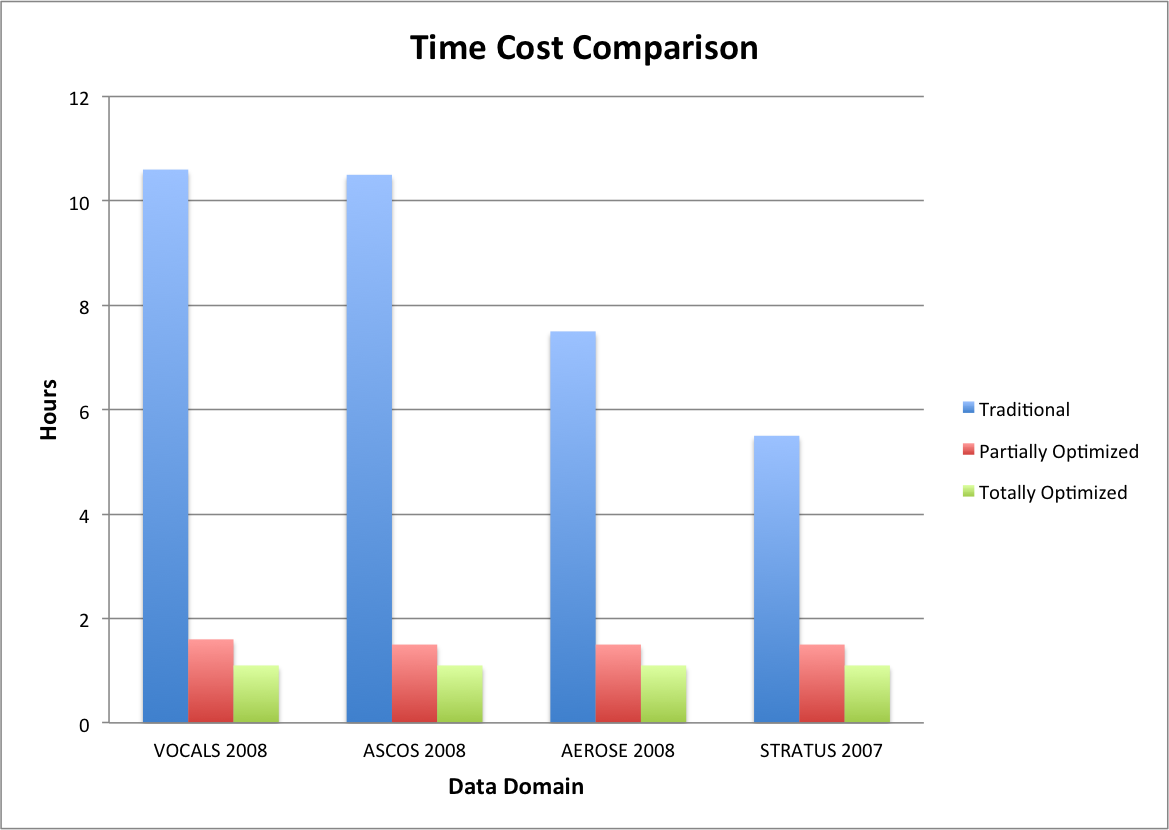
\includegraphics[scale=0.6]{TimeComp.png}
  \caption{Execution Time Comparison}
  \label{fig:TCC}
\end{center}
\end{figure}

\begin{table}[!iht]
\centering
\begin{tabular}{|c|c|c|c|p{3cm}|}
\hline
\textbf{Data Domain} & \textbf{Total Size} &\textbf{ Service Request \& Response (Hrs)}  & \textbf{Discovery Histogram (Mins)} & \textbf{Total Execution Time (Hrs)}  \\ \hline
VOCALS 2008 &  $\sim$3920 MB & $\sim$1 & $\sim$7.221 & $\sim$1.1\\ \hline
ASCOS 2008 & $\sim$3500 MB & $\sim$1 & $\sim$6.379& $\sim$1.1\\ \hline 
AEROSE 2008 & $\sim$2880 MB & $\sim$1 & $\sim$6.218&  $\sim$1.1 \\\hline 
STRATUS 2007 & $\sim$1470 MB & $\sim$1  & $\sim$6.019&  $\sim$1.1\\\hline
\end{tabular}
\caption{ Execution time of applying the service-oriented histogram with on-demand sorting approach to implement discovery histogram}
\label{tbl:3rdStr}
\end{table}

\end{enumerate}

Figure \ref{fig:TCC} shows the comparison of execution time the three different histogram approaches. From the figure, we can see the execution time of discovery histogram for all the four projects' data sets have been reduced tremendously in terms of execution time. 

\section{Conclusion and Future Work}
Climate data is well known for its tremendous size of data sets, which creates many challenges for visualizing global and local data sets with acceptable performance. In this paper, we propose a novel approach, named Service-Oriented Histogram with On-demand Sorting, that embraces the concepts and benefits of SOA to address the performance problems of data transferring and data navigation (drill-up and drill-down). To evaluation our approach, we conduct experiments on comparing the performance of three histogram approaches on implementing discovery histogram: traditional histogram, service-oriented histogram, and service-oriented histogram with on-demand sorting. Our preliminary results show that our service-oriented histogram with on-demand sorting approach achieve the best performance, which significantly reduce the execution time for data transferring and data navigation. Due to time limitation, we do not conduct complehensive experiments on larger size data sets. We plan to conduct such experiments so that we can better evaluate our approaches and improve the approaches.

\bibliographystyle{unsrt}
\bibliography{references}
\end{document}